\documentclass[12pt, a4paper, oneside, openright]{book}
\pdfpagewidth\paperwidth
\pdfpageheight\paperheight
\usepackage{graphicx}
\usepackage{subfigure}
\usepackage{hyperref}
\usepackage{amsmath}
\usepackage{amsthm}
\usepackage{amsfonts}
\usepackage{amssymb}
\frenchspacing
\makeatletter
\let\@orig@endthebibliography\endthebibliography 
\renewcommand\endthebibliography{% 
  \xdef\@kept@last@number{\the\c@enumiv}% 
  \@orig@endthebibliography} 

\newenvironment{thesitography}[1] 
  {\def\bibname{Sitografia}% 
   \thebibliography{#1}% 
   \setcounter{enumiv}{\@kept@last@number}% 
} 
  {\@orig@endthebibliography} 
\makeatother
\begin{document}
\pagestyle{myheadings}
\begin{titlepage}
\begin{center}
{{\Large{\textsc{Universit\`{a} degli studi di Firenze}}}} \rule[0.1cm]{15.8cm}{0.1mm}
\rule[0.5cm]{15.8cm}{0.6mm}
{\small{\bf SCUOLA DI INGEGNERIA\\
Corso di Laurea Magistrale in Ingegneria Informatica}}
\end{center}
\vspace{15mm}
\begin{center}
{\LARGE{\bf Testing of chosen Design Patterns}}\\
\vspace{3mm}
{\LARGE{\bf with JUnit and Mockito}}\\
\end{center}
\begin{figure}
\centering

\includegraphics[scale=0.2]{./LaTeX_extra/logo-unifi-1.png}
\end{figure}
\vspace{32mm}
\par
\noindent
\begin{minipage}[t]{0.55\textwidth}
{\large{\bf Docente\\
Prof. Enrico Vicario}} \\
\end{minipage}
\hfill
\begin{minipage}[t]{0.47\textwidth}\raggedleft
{\large{\bf Relazione a cura di\\
Niccolo' Fabbri\\
Francesco Santoni}}
\end{minipage}
\vspace{12mm}
\vspace{12mm}
\begin{center}
{\large{\bf Firenze,\\%inserire il numero della sessione in cui ci si laurea
24 Agosto 2016 }}%inserire l'anno accademico a cui si è iscritti
\end{center}
\end{titlepage}

\mainmatter
\pagenumbering{roman}
\newpage\null\thispagestyle{empty}
\null\vspace{\stretch{0.6}}
\pagenumbering{gobble}
\frontmatter
\clearpage
\tableofcontents
\cleardoublepage
\mainmatter

\chapter{Introduction}
\markboth{Introduction}{\textit{Introduction}}

We identify a collection of structural and behavioral design patterns: Class Adapter, Object Adapter, Proxy, Decorator, Composite, Observer, State, Visitor.

% ordine degli strutturali � individuato dalla "naturale" evoluzione in complessit� della topologia% 
For each pattern we realize an implementation in Java and we develop a reasoned test suite based on a realistic fault model and on chosen coverage criteria.

We realize the tests through the JUnit\cite{1} plug-in for Eclipse and the Mockito\cite{2} framework. EclEmma \cite{3} is used to provide a code coverage measure.


\chapter{Design Patterns}
\markboth{Design Patterns}{\textit{Design Patterns}}
In software engineering, a software design pattern is a general reusable template to solve a commonly occurring problem within a given context.

We will study:
\begin{enumerate}
	\item Structural patterns: Adapter(both in his Class and Object variants), Proxy, Decorator, Composite.
	\item Behavioural patterns: Observer, State, Visitor.
\end{enumerate}


\section{Class Adapter}
 Adapts a pre-existent class to a new interface through inheritance. 
 
 Through the new interface the old methods can be directly presented, modified, produce aggregated results or completely new functionality can be added. 
 
 
\subsubsection{Class Diagram}
\begin{figure}[!h]
	\centering
	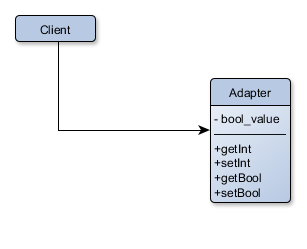
\includegraphics[width=0.6\textwidth]{./Adapter/Class/ClassDiagram.png}
	\caption{Class Adapter: Class Diagram }
	\label{CAclassDiag}
\end{figure}

\begin{itemize}
	\item \textbf{Adaptee}: legacy class with specific methods and fields
	\item \textbf{Target}: desired interface
	\item \textbf{ClassAdapter}: inherits from both Adaptee and Target, adapts the legacy methods to the desired interface  
\end{itemize}

\subsubsection{Fault Model}
Given that the pattern focuses on allowing access to legacy methods through a new interface, failures are found in the following situations:  
\begin{itemize}
	\item the adapter did not inherit from the legacy class or the new interface
	\item the adapter for some reason cannot interact with the legacy methods 
\end{itemize}

\subsection{Testing}
The two sources of failure both depend on the inability of the Client to reach the Adaptee methods through the Adapter.  We reasoned that it is thus sufficient to test the ways in which the variable \textit{bool\_value} interacts and is modified by the methods.

 As long as the variable changes in an unexpected way the connection between Client and Adaptee is in fact cut off.
\newline
We have thus represented the field's interaction with the class methods through a data flow graph in which the granularity was set such that basic blocks are represented by functions.

We then decided to test the interaction between the variable and the methods following the\textit{ all-uses} criterion, we in fact deemed the\textit{ all-def} criterion not useful to test this pattern because we value mainly the transmission of the right value of the field and thus all its \textit{uses}.    


\paragraph{Data Flow Graph}
 The Client is the only external class interacting with the public methods of the Adapter. The Data Flow Graph can be seen in Figure \ref{CAdataflow}.
\begin{figure}[h]
	\centering
	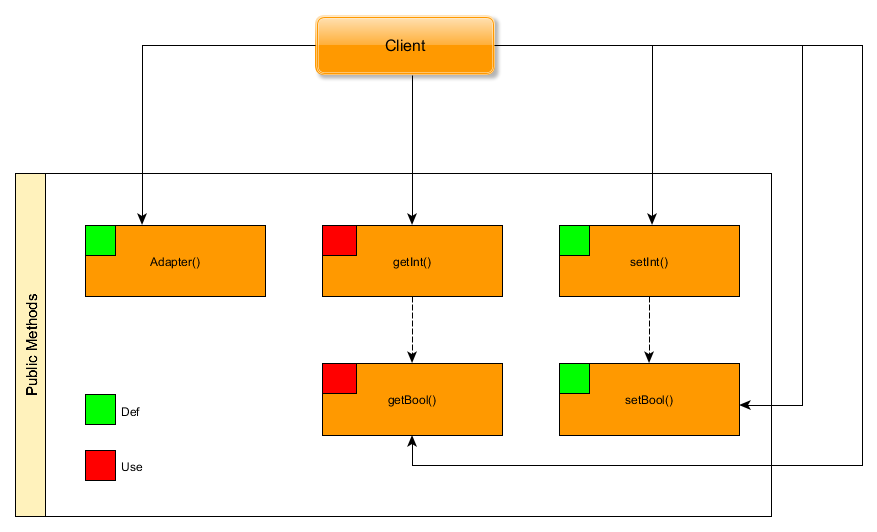
\includegraphics[width=0.8\textwidth]{./Adapter/Class/CallGraph.png}
	\caption{Data Flow Graph: \textit{bool\_value}}
	\label{CAdataflow}
\end{figure}


\subsubsection{Tests}
We generated a test suite capable of testing all the \textit{all-uses} paths:
\begin{itemize}
	\item Adapter() getInt() 
	\item Adapter() getBool() 
	\item Adapter() setInt() getInt() 
	\item Adapter() setInt() getBool() 
	\item Adapter() setBool() getInt()
	\newline
\end{itemize}
The special case of
\begin{itemize}
	\item Adapter() setBool() getBool() 
		
\end{itemize}	
is not tested because all the methods are directly inherited from the legacy class(and thus are supposedly already tested) and no side-effects, which could have invalidated some invariants, are introduced in the adapter.

In this particular pattern the presence of a lone object other than the Client makes Unit and Integration tests un-distinguishable.

\subsubsection{Code Coverage}
The code coverage measure obtained from EclEmma Java plug-in is: 100\%.

%%%%%%%%%%%%%%%%%%%%%%%%%%%%%%%%%%%%%%%%%%%%%1
\section{Object Adapter}
Adapts a pre-existent class to a new interface through class composition. 

Through the new interface the old methods can be directly presented, modified, produce aggregated results or completely new functionality can be added. 

The composition adds the possibility of dynamically switching the adapted legacy class (not contemplated in our implementation) and the possibility of overridden methods with altered functionality.

If the adaptee class is declared final, the increased complexity from overridden methods is eliminated but the extra functionality is removed as well.


\subsubsection{Class Diagram}
\begin{figure}[!h]
	\centering
	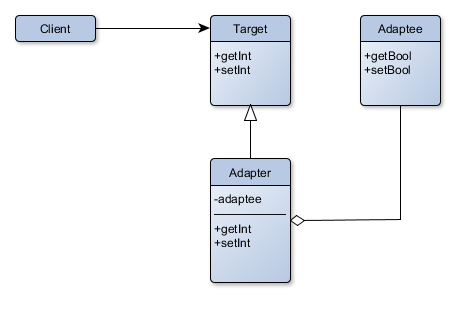
\includegraphics[width=0.7\textwidth]{./Adapter/Object/ClassDiagram.png}
	\caption{Object Adapter: Class Diagram }
	\label{OAclassDiag}
\end{figure}

\begin{itemize}
	\item \textbf{Adaptee}: legacy class with specific methods and fields
	\item \textbf{Target}: desired interface
	\item \textbf{ObjectAdapter}: inherits from Target, adapts the legacy methods to the desired interface through delegation. 
\end{itemize}

\subsubsection{Fault Model}
Given that the pattern focuses on allowing access to legacy methods through a new interface, failures are found in the following situations:  
\begin{itemize}
	\item the adapter did not inherit from the legacy class or the new interface
	\item the adapter for some reason cannot interact with the legacy methods 
	\item the instance contained in the adapter, which inherited the adaptee class, has overrode its methods in an unforeseen way
\end{itemize}


\subsection{Testing}

The sources of failure depend on the inability of the Client to reach the Adaptee methods through the Adapter or in the inability of the Adapter in foreseeing the possible ways in which the Adaptee methods can be overridden:  we reasoned that it is sufficient to test the ways in which the variable \textit{bool\_value} interacts and is modified by the methods, considering all the possible alternative implementations. 
As long as the variable changes in an unexpected way the connection between Client and Adaptee is in fact cut off.

The problem of testing thus expands in two different orthogonal dimensions: data flow, the series of calls that modify or use the variable\textit{bool\_value},  and topology, the different ways the classes are ordered in a hierarchy at runtime.

We decided to explore both of them separately in specific focused tests.
\newline
\paragraph{Field \textit{adaptee}: Data flow}
We have represented the field's interaction with the class methods through a data flow graph in which the granularity was set such that basic blocks are represented by functions.

\subparagraph{Data Flow Graph}
Like the ClassAdapter, only the Client interacts with the Adapter methods.
The Data Flow Graph can be seen in Figure \ref{OAdataflow}.
\begin{figure}[!h]
	\centering
	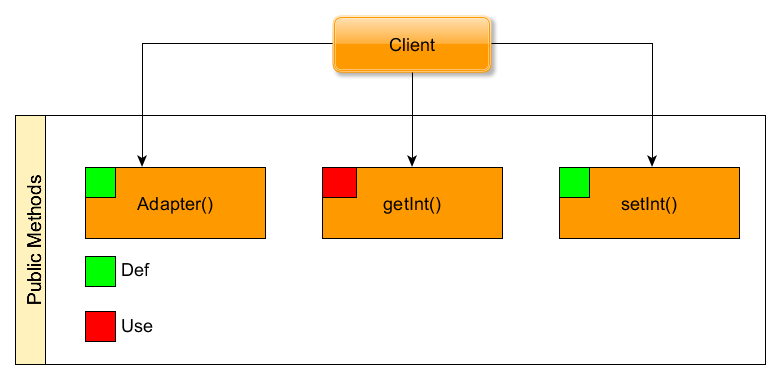
\includegraphics[width=0.8\textwidth]{./Adapter/Object/CallGraph.png}
	\caption{Data Flow Graph: \textit{bool\_value}}
	\label{OAdataflow}
\end{figure}


We then decided to test the interaction between the variable and the methods following the\textit{ all-uses} criterion, we in fact deemed the \textit{all-def} criterion not useful to test this pattern because we value mainly the transmission of the right value of the field and thus all its \textit{uses}.   

\paragraph{Overridden methods: Topology}
We have tested separately the overridden variants of the methods through simple tests.

We reasoned that such a separation would allow us to sufficiently cover the code while maintaining a low number of tests.

\subsubsection{Tests}



We generated a test suite capable of testing all the \textit{all-uses} paths:
\begin{enumerate}
	\item Adapter() getInt() 
	\item Adapter() setInt() getInt() 
	
\end{enumerate}
To these are also added the topology tests:
\begin{enumerate}
	\item Adapter( Adaptee ) getInt() 
	\item Adapter( AdapteeOpposite ) getInt()
\end{enumerate}	
Of these the first, being already tested in the first suite, is not repeated.

Since in this pattern the tested class's methods (Adapter's) interacted with external classes (Adaptee) we  differentiated between Unit and Integration tests.

We utilized Mockito's \textit{mock} function to isolate errors with an origin in external classes from interfering with the Adapter class's code.
\subsubsection{Code Coverage}
The code coverage measure obtained from EclEmma Java plugin is: 98.6\% 
\begin{itemize}
	\item Adapter: 97.1\% (UnitTest: 97.1\%)
	\item Adaptee: 100\%
	\item AdapteeOpposite: 100\% 
\end{itemize}

The single remaining untested branch is a setter method which was not called with all the possible inputs equivalence classes.

Since the Unit Tests and the Integration Tests are identical, with the only difference that the Unit Tests utilize Mockito's help to isolate from external classes, the coverage of the Adapter class's code is the same.

%%%%%%%%%%%%%%%%%%%%%%%%%%%%%%%%%%%%%%%%%%%%%2

\section{Proxy}

The Proxy pattern is constituted by a class  functioning as an interface to something else, usually a complex or heavy object.

 It is called by the client to access the real serving object behind the scenes, it either provides a cached result or transmits the request to the actual object.

\subsubsection{Class Diagram}
\begin{figure}[!h]
	\centering
	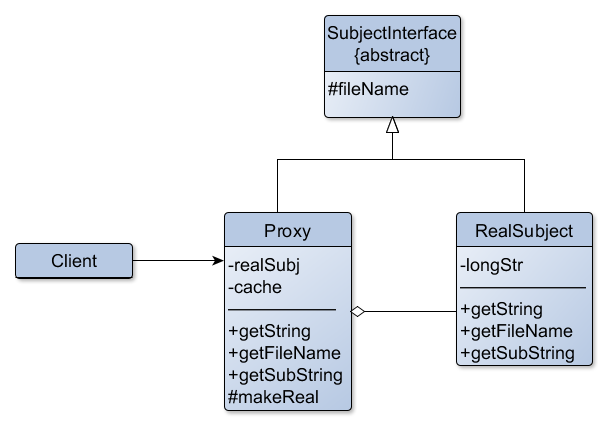
\includegraphics[width=0.7\textwidth]{./Proxy/ClassDiagram.png}
	\caption{Proxy: Class Diagram }
	\label{ProclassDiag}
\end{figure}

\begin{itemize}
	\item \textbf{SubjectInterface}: defines the interface used by the Client to access the RealSubject.
	\item \textbf{Proxy}: allows access to the RealSubject, either by providing a cached response or by delegating the requests to the RealSubject itself.
	\item \textbf{RealSubject}: defines the real complex or heavy object wrapped by the proxy.
\end{itemize}

\subsubsection{Fault Model}

The pattern focuses on optimizing or controlling the access to the heavy subject. We have failures in the following situations:  
\begin{itemize}
	\item the access to the RealSubject is impeded
	\item the cached copies provided by the wrapper differ from the actual source.
\end{itemize}

\subsection{Testing}

The sources of failure depend on the inability of the Client to reach the RealSubject fields through the Proxy or in the inability of the Proxy of providing correct cached versions:  we reasoned that it is sufficient to test the ways in which the variable \textit{realSubj} interacts and is modified by the methods, by slight modification of the tests we can automatically verify the cached versions validity.




\paragraph{Field \textit{price}: Data flow}
We have represented the field's interaction with the class methods through a data flow graph in which the granularity was set such that basic blocks are represented by functions.

\subparagraph{Data Flow Graph}
Only the Client interacts with the Proxy methods.
The Data Flow Graph can be seen in Figure \ref{Prodataflow}.
\begin{figure}[!h]
	\centering
	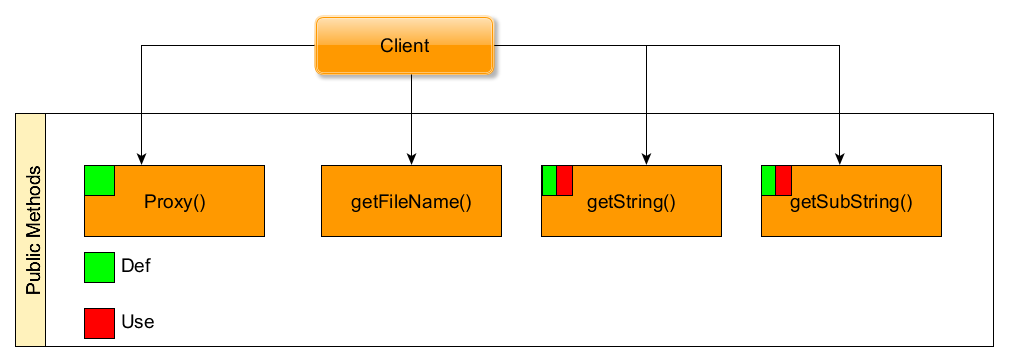
\includegraphics[width=0.8\textwidth]{./Proxy/CallGraph.png}
	\caption{Data Flow Graph: \textit{realSubj}}
	\label{Prodataflow}
\end{figure}


We decided to test the interaction between the variable and the methods following the\textit{ all-uses} criterion, we in fact desired to verify through the tests not only the correct interactions of the \textit{realSubj} field with the methods but also the \textit{cache}'s, we determined that a more extensive coverage could thus be desired.

\subsubsection{Tests}

\paragraph{Field \textit{price}: Data flow}
We generated a test suite capable of testing all the \textit{all-uses} paths:
\begin{enumerate}
	\item Proxy() getString() 
	\item Proxy() getString() getString()
	\item Proxy() getSubString()
	\item Proxy() getString() getSubString()
	\item Proxy() getSubString() getSubString()
	\item Proxy() getSubString() getString()
	
\end{enumerate}
In particular  \textit{Proxy() getSubString() getSubString()} was altered to test the returned cached version after each method call. 


Since in this pattern the tested class's methods (Proxy's) interacted with external classes (RealSubject) we  differentiated between Unit and Integration tests.

The Proxy class, by having to provide a cached version or to instantiate a RealSubject which will process the heavy data and return it to the Proxy, poses problems to the injection of a mocked RealSubject class.

Two possibilities were considered: create a RealSubjectFactory to pass during the construction of the Proxy and utilize it during the instantiation of the inner RealSubject or separate the responsibility of instantiation in a method void of logic.

In the first possibility one would have to use Mockito's \textit{mock} method to mock the Factory so that it would return a mocked RealSubject, while in the second case one would have to use Mockito's \textit{spy} method to modify the Proxy itself so that the logic-less method would return a mocked RealSubject.

Due to not having to create an unnecessary extra class we preferred and thus implemented the second option.

\subsubsection{Code Coverage}
The code coverage measure obtained from EclEmma Java plugin is: 93.8\% 
\begin{itemize}
	\item Proxy: 95.4\% (UnitTest 95.4\%)
	\item RealSubject: 88\%
	\item SubjectInterface: 100\%
	
\end{itemize}

The remaining untested branches correspond to the \textit{getFilename()} methods, which where not tested due to absence of logic.

Since the Unit Tests and the Integration Tests are identical, with the only difference that the Unit Tests utilize Mockito's help to isolate from external classes, the coverage of the Proxy class's code is the same.
%%%%%%%%%%%%%%%%%%%%%%%%%%%%%%%%%%%%%%%%%%%%%3
\section{Decorator}

%%%%%%%%%%%%%%%%%%%%%%%%%%%%%%%%%%%%%%%%%%%%%4
\section{Composite}

The Composite pattern "composes" objects into tree structures to represent part-whole hierarchies. Implementing the composite pattern lets clients treat individual objects and compositions uniformly.

\subsubsection{Class Diagram}
\begin{figure}[!h]
	\centering
	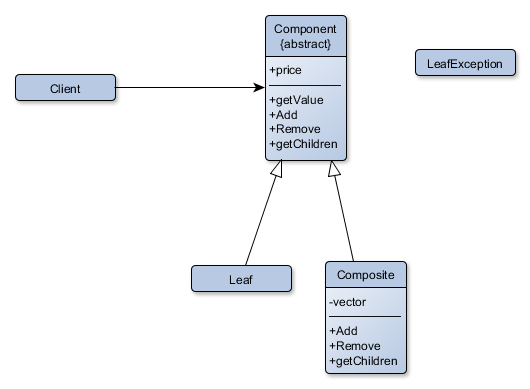
\includegraphics[width=0.7\textwidth]{./Composite/ClassDiagram.png}
	\caption{Composite: Class Diagram }
	\label{CoclassDiag}
\end{figure}

\begin{itemize}
	\item \textbf{Component}: common interface to the individual and compound objects.
	\item \textbf{Composite}: composition of individual objects and other compositions.
	\item \textbf{Leaf}: individual object. 
	\item \textbf{LeafException}: exception thrown when a composite-specific method is called on a Leaf object. 
		
\end{itemize}

\subsubsection{Fault Model}

The pattern focuses on treating uniformly individual and compound objects. Grave errors are found in the following situations:  
\begin{itemize}
	\item the common \textit{operation} works differently than expected
	\item the composite-specific methods produce unexpected effects when called on a Leaf object
\end{itemize}


\subsection{Testing}

The sources of failure depend on the inability of the specific components (individual or composite parts) to be interacted in an uniform way. We reasoned that to produce a satisfying test suite we must test two different things: the way \textit{operation} works under the possible hierarchies at runtime and the way the different objects behave under calls from composite-specific methods.

As long as outcomes different from the expectation are observed we can reasonably predict that no uniform treatments of the components is in place.

The problem of testing thus expands in two different orthogonal dimensions: data flow, the series of calls that modify or use the variable\textit{price},  and topology, the different hierarchies of objects with respect to the method \textit{operation}.


We decided to explore both of them separately in specific focused tests.
\newline
\paragraph{Field \textit{price}: Data flow}
We have represented the field's interaction with the class methods through a data flow graph in which the granularity was set such that basic blocks are represented by functions.

\subparagraph{Data Flow Graph}
Both Client and other wrapping Composites interacts with the Component methods.
The Data Flow Graph can be seen in Figure \ref{Codataflow}.
\begin{figure}[!h]
	\centering
	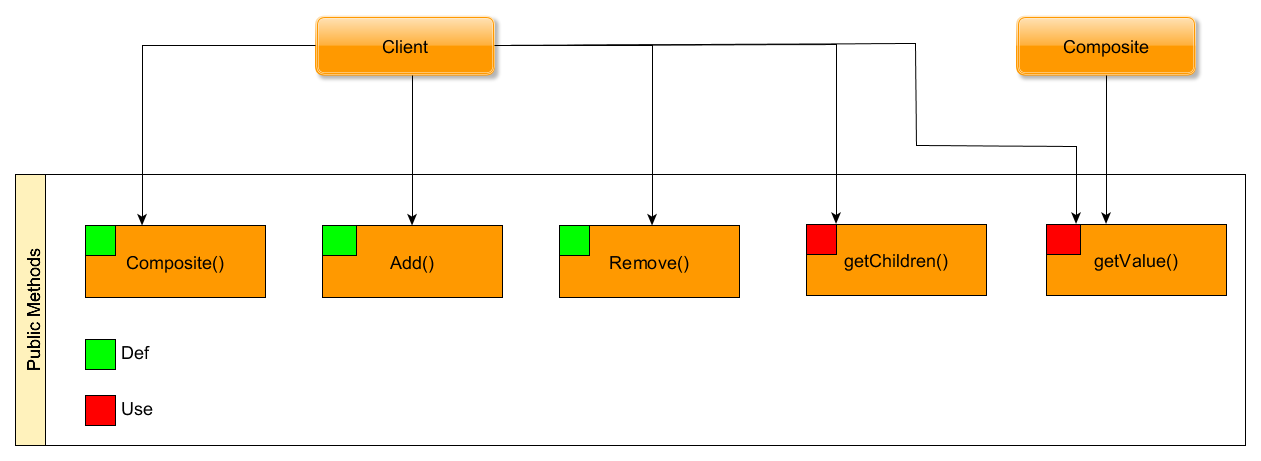
\includegraphics[width=0.8\textwidth]{./Composite/CallGraph.png}
	\caption{Data Flow Graph: \textit{price}}
	\label{Codataflow}
\end{figure}


We then decided to test the interaction between the variable and the methods following the\textit{ all-uses} criterion, we deemed the \textit{all-def} criterion excessively restrictive to test this pattern.

The field was tested in the fixed hierarchy formed with a Composite element containing another Composite, which contained a Leaf.  
We reasoned that the chosen fixed hierarchy, while not allowing to test on each possible instance, is sufficiently complete, maintaining a balance between number of tests and efficiency.
  
  
  
\paragraph{Method \textit{operation\(\)}: Topology}
We generated a Class Dependency Graph to identify all the possible relations between classes.

\subparagraph{Class Dependency Graph}
In the Figure \ref{Codepengraph} are made explicit the relations between classes: in particular since Component is an abstract class it and its inheriting classes depend on each other. 
\begin{figure}[!h]
	\centering
	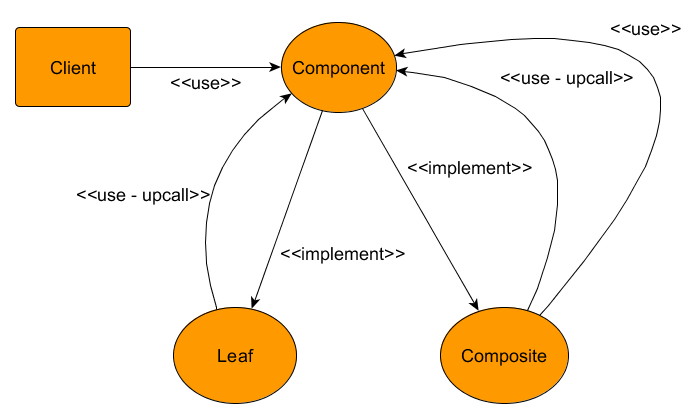
\includegraphics[width=0.8\textwidth]{./Composite/ClassDepencyGraph.png}
	\caption{Data Flow Graph: \textit{operation()}}
	\label{Codepengraph}
\end{figure}

We decided to generate a test suite dependent on the \textit{all-edges} criterion.\textit{ all-nodes} is in fact excessively relaxed and would not cover all cases of interests. 

\subsubsection{Tests}

\paragraph{Field \textit{price}: Data flow}
We generated a test suite capable of testing all the \textit{all-uses} paths:
\begin{itemize}
	\item Component() getChild()
	\item Component() getValue()
	\item Component() add() getChild()
	\item Component() add() getValue()
	\item Component() add() add() remove() getChild()
	\item Component() add() add() remove() getValue() 
\end{itemize}

\paragraph{Method \textit{operation\(\)}: Topology}
We identified the 3 cases of:
\begin{itemize}
	\item single Leaf
	\item Composite containing Leaf
	\item Composite containing Composite
\end{itemize}
as representative of the entire set of possible hierarchies.

We then tested all the composite-specific methods (add, remove, getChild) on the identified cases.

In both type of tests, since the tested class's methods (Component) interacted with external classes (Leaf or Composites) we  differentiated between Unit and Integration tests.

We utilized Mockito's \textit{mock} function to isolate errors with an origin in external classes from interfering with the main class's code.
\subsubsection{Code Coverage}
The code coverage measure obtained from EclEmma Java plugin is: 97.8\% 
\begin{itemize}
	\item Component: 92.3\% (UnitTest 92.3\%)
	\item Composite: 100\%
	\item Leaf: 100\%
	\item LeafException 100\%
\end{itemize}

The remaining untested branches are found in the implementation of the composite-specific methods that Component provides for Leaf: all other classes (Composite) directly override those methods so their implementation when they are called not by a Leaf is never tested.

Since the Unit Tests and the Integration Tests are identical, with the only difference that the Unit Tests utilize Mockito's help to isolate from external classes, the coverage of the classes' code is the same.


%%%%%%%%%%%%%%%%%%%%%%%%%%%%%%%%%%%%%%%%%%%%%5
\section{Observer}

In the Observer pattern an object, called the subject, maintains a list of its dependents, called observers, and notifies them automatically of any state changes, usually by calling one of their methods.

The observers must be explicitly associated and disassociated with the subjects they follow, possibly causing memory leaks.

\subsubsection{Class Diagram}
\begin{figure}[!h]
	\centering
	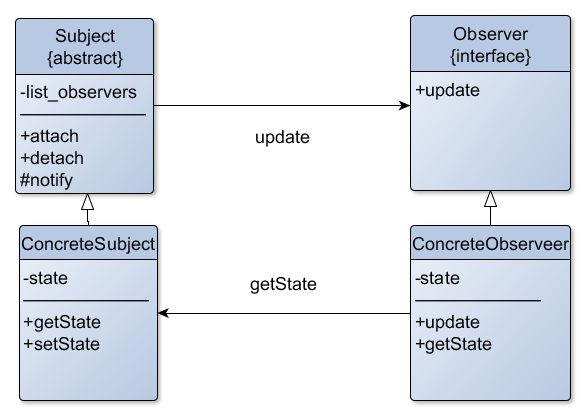
\includegraphics[width=0.7\textwidth]{./Observer/ClassDiagram.png}
	\caption{Observer: Class Diagram }
	\label{ObclassDiag}
\end{figure}

\begin{itemize}
	\item \textbf{Subject}: provides methods to add or remove observers in his list of followers.
	\item \textbf{Observer}: specifies an interface for the notification of change on a subject.
	\item \textbf{ConcreteSubject}: contains a state that can be modified. 
	\item \textbf{ConcreteObserver}: implements the update operation. 
	
\end{itemize}

\subsubsection{Fault Model}

The pattern focuses on maintaining updated objects that expressed the interest in a specific subject. Failures are found in the following situations:  
\begin{itemize}
	\item \textit{attach} and \textit{detach} do not produce the expected results.
	\item after a change of the subject state the following observers are not \textit{notified}.
	\item the observer after being notified does not execute correctly the \textit{update} method.
\end{itemize}


\subsection{Testing}

The sources of failure depend on the presence of problems that impede the correct functioning of the inter-class methods and, in the lesser part, by the inability of the observer to correctly update. We considered the correct modification on the subject internal \textit{state} as not important for our pattern.  We reasoned that to produce a satisfying test suite we must test the way \textit{list\_observers} is modified after an inter-class method invocation and the way the \textit{state} of the observer is modified after a notification.



As long as the outcomes differ from the expectation we can reasonably predict that the transmission of information upon notification encountered problems.

\paragraph{Field \textit{list\_observers}: Data flow}
We have represented the field's interaction with the class methods through a data flow graph in which the granularity was set such that basic blocks are represented by functions.

\subparagraph{Data Flow Graph}
Only the Client interacts with the Subject methods, in particular the responsibility of attaching or detaching Observers from Subjects lies with the Client.
The Data Flow Graph can be seen in Figure \ref{Obdataflow1}.
\begin{figure}[!h]
	\centering
	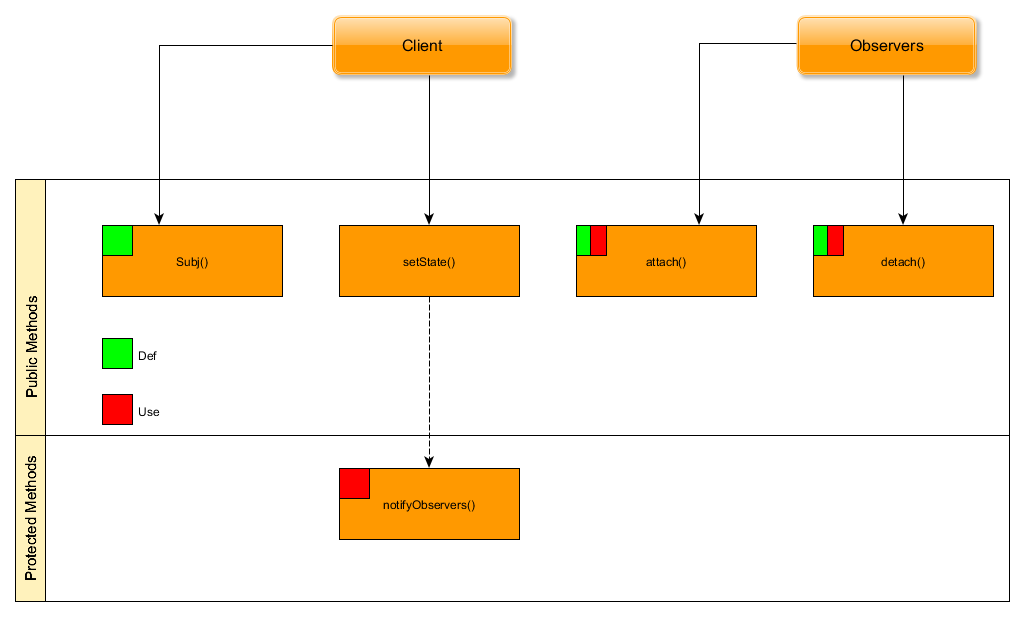
\includegraphics[width=0.8\textwidth]{./Observer/CallGraph.png}
	\caption{Data Flow Graph: \textit{list\_observers}}
	\label{Obdataflow1}
\end{figure}


We decided to test the interaction between the variable and the methods following the\textit{ all-uses} criterion.

\paragraph{Field \textit{state}: Data flow}
We have represented the field's interaction with the class methods through a data flow graph in which the granularity was set such that basic blocks are represented by functions.

\subparagraph{Data Flow Graph}
Both Client and followed Subjects interacts with the Component methods.
The Data Flow Graph can be seen in Figure \ref{Obdataflow2}.
\begin{figure}[!h]
	\centering
	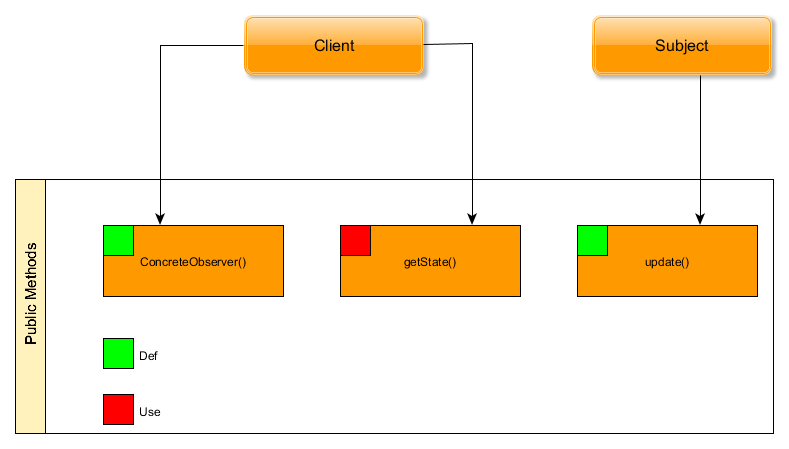
\includegraphics[width=0.8\textwidth]{./Observer/CallGraph_State.png}
	\caption{Data Flow Graph: \textit{state}}
	\label{Obdataflow2}
\end{figure}


We decided to test the interaction between the variable and the methods following the\textit{ all-uses} criterion, we deemed the \textit{all-def} criterion excessively restrictive to test this pattern.


\subsubsection{Tests}

\paragraph{Field \textit{list\_observer}: Data flow}
We decided to test as separate and distinct cases for situations like \textit{detach() detach()} where the methods are called with the same Observer or different ones. 
We generated a test suite capable of testing all the \textit{all-uses} paths:
\begin{enumerate}
	\item Subject() setState()[notify()]	
	\item Subject() detach() 		
	\item Subject() attach()x3 detach()x2 (+setState()[notify()]) 
	\item Subject() attach()x2 detach()x2 attach() detach() attach() (+setState()[notify()])
\end{enumerate}

All these paths are interesting to study:
\begin{enumerate}
	\item controls no errors are introduced if a \textit{setState()} is called with empty list
	\item a detach is called with empty list
	\item[3,4] by interspersing verifications on the \textit{list\_observer} we test all combinations of the different D-U paths:
	\begin{enumerate}
		\item attach() attach()  
		\item attach() detach()	 	
		\item detach() detach()	 
		\item detach() notify()
		\item Subject() attach()
		\item detach() attach()
		\item attach() notify()
	\end{enumerate} 
	
\end{enumerate} 
To create an output of the \textit{list\_observer} we utilize a support method void of logic, which we decided did not need to be considered as an \textit{use} during the tests.


\paragraph{Field \textit{state}: Data flow}
We generated a test suite capable of testing all the \textit{all-uses} paths:
\begin{enumerate}
	\item ConcreteObserver() getState()
	\item ConcreteObserver() update() getState()
	
\end{enumerate}
	

	

In both type of tests, since the tested class's methods (ConcreteSubject and ConcreteObserver) interacted with external classes (Observer and Subject) we  differentiated between Unit and Integration tests.

We utilized Mockito's \textit{mock} function to isolate errors with an origin in external classes from interfering with the main class's code.
To 
\subsubsection{Code Coverage}
The code coverage measure obtained from EclEmma Java plugin is: 100\% (Unit: 100\%)


%%%%%%%%%%%%%%%%%%%%%%%%%%%%%%%%%%%%%%%%%%%%%6
\section{State}

%%%%%%%%%%%%%%%%%%%%%%%%%%%%%%%%%%%%%%%%%%%%%7
\section{Visitor}


non era necessario la Answer  es.particolare logica che decide che fare(avrei potuto lo stesso chiamare direttamente con cast, forse testando di piu anche) si e' deciso di esplorare le potenzialita' di Mockito..
%%%%%%%%%%%%%%%%%%%%%%%%%%%%%%%%%%%%%%%%%%%%%8

\chapter{JUnit \& Mockito}

\section{JUnit}
\section{Mockito}
answer serve per fare cose complesse es. particolare logica che decide che fare, qui lo ho usato per cose banali


\paragraph{EclEmma}
EclEmma is a plug-in which measures the branch coverage of the bytecode produced by the compiler. The branches which were not tested are then traced back to the code and highlighted as a warning. 

In some cases such highlighting is confusing and can even be impossible to eliminate through testing: the Java compiler in fact sometimes creates additional bytecode that seems to have no relation to the source code (e.g. synthetic classes and methods). 

In some other cases test execution is questionable or impossible by design: for example private, empty default constructors (assuming they receive no calls) or methods that contains no logic, like plain getters and setters,
or even extra exception handlers installed to close resources from try/with statements.

\chapter{Conclusioni}

In questo elaborato abbiamo mostrato un sistema in grado di riconoscere automaticamente i muri di una planimetria, indipendentemente dalla notazione grafica utilizzata. In questo programma, se i muri rientrano nelle tipologie citate, � indipendente dagli altri standard e non necessita di informazioni aggiuntive per svolgere il proprio compito.
Dalla bont� dei risultati mostrati nel paragrafo precedente si pu� notare che quello presentato � un metodo valido per l'individuazione di muri in planimetrie. Le idee di base, in parte ispirate agli articoli \cite{1} e \cite{5} e in parte sviluppate ex novo, si sono dimostrate valide per raggiungere l'obiettivo prefissato. A sostegno di quanto appena detto viene ricordato quanto riportato nel capitolo precedente: ossia il fatto che i nostri risultati sono molto simili a quelli ottenuti da CVC ed in alcuni casi sono risultati anche migliori.
Con l'utilizzo di queste idee appena esposte sarebbe possibile arrivare ad un riconoscimento al 100\% indipendente dagli standard grafici utilizzati solo con un'aggiunta di codice che, riconosciuti i muri non pieni, si limiti a riempirli. Una volta raggiunto questo obiettivo un altro sviluppo futuro potrebbe essere il riconoscimento (gi� effettuato da CVC) di altri elementi strutturali quali porte, finestre e stanze.

\addcontentsline{toc}{chapter}{Bibliografia}
\begin{thebibliography}{99}

\bibitem{1} 

\end{thebibliography}
\addcontentsline{toc}{chapter}{Elenco delle Figure}\listoffigures
\end{document}
